\documentclass[1p]{elsarticle_modified}
%\bibliographystyle{elsarticle-num}

%\usepackage[colorlinks]{hyperref}
%\usepackage{abbrmath_seonhwa} %\Abb, \Ascr, \Acal ,\Abf, \Afrak
\usepackage{amsfonts}
\usepackage{amssymb}
\usepackage{amsmath}
\usepackage{amsthm}
\usepackage{scalefnt}
\usepackage{amsbsy}
\usepackage{kotex}
\usepackage{caption}
\usepackage{subfig}
\usepackage{color}
\usepackage{graphicx}
\usepackage{xcolor} %% white, black, red, green, blue, cyan, magenta, yellow
\usepackage{float}
\usepackage{setspace}
\usepackage{hyperref}

\usepackage{tikz}
\usetikzlibrary{arrows}

\usepackage{multirow}
\usepackage{array} % fixed length table
\usepackage{hhline}

%%%%%%%%%%%%%%%%%%%%%
\makeatletter
\renewcommand*\env@matrix[1][\arraystretch]{%
	\edef\arraystretch{#1}%
	\hskip -\arraycolsep
	\let\@ifnextchar\new@ifnextchar
	\array{*\c@MaxMatrixCols c}}
\makeatother %https://tex.stackexchange.com/questions/14071/how-can-i-increase-the-line-spacing-in-a-matrix
%%%%%%%%%%%%%%%

\usepackage[normalem]{ulem}

\newcommand{\msout}[1]{\ifmmode\text{\sout{\ensuremath{#1}}}\else\sout{#1}\fi}
%SOURCE: \msout is \stkout macro in https://tex.stackexchange.com/questions/20609/strikeout-in-math-mode

\newcommand{\cancel}[1]{
	\ifmmode
	{\color{red}\msout{#1}}
	\else
	{\color{red}\sout{#1}}
	\fi
}

\newcommand{\add}[1]{
	{\color{blue}\uwave{#1}}
}

\newcommand{\replace}[2]{
	\ifmmode
	{\color{red}\msout{#1}}{\color{blue}\uwave{#2}}
	\else
	{\color{red}\sout{#1}}{\color{blue}\uwave{#2}}
	\fi
}

\newcommand{\Sol}{\mathcal{S}} %segment
\newcommand{\D}{D} %diagram
\newcommand{\A}{\mathcal{A}} %arc


%%%%%%%%%%%%%%%%%%%%%%%%%%%%%5 test

\def\sl{\operatorname{\textup{SL}}(2,\Cbb)}
\def\psl{\operatorname{\textup{PSL}}(2,\Cbb)}
\def\quan{\mkern 1mu \triangleright \mkern 1mu}

\theoremstyle{definition}
\newtheorem{thm}{Theorem}[section]
\newtheorem{prop}[thm]{Proposition}
\newtheorem{lem}[thm]{Lemma}
\newtheorem{ques}[thm]{Question}
\newtheorem{cor}[thm]{Corollary}
\newtheorem{defn}[thm]{Definition}
\newtheorem{exam}[thm]{Example}
\newtheorem{rmk}[thm]{Remark}
\newtheorem{alg}[thm]{Algorithm}

\newcommand{\I}{\sqrt{-1}}
\begin{document}

%\begin{frontmatter}
%
%\title{Boundary parabolic representations of knots up to 8 crossings}
%
%%% Group authors per affiliation:
%\author{Yunhi Cho} 
%\address{Department of Mathematics, University of Seoul, Seoul, Korea}
%\ead{yhcho@uos.ac.kr}
%
%
%\author{Seonhwa Kim} %\fnref{s_kim}}
%\address{Center for Geometry and Physics, Institute for Basic Science, Pohang, 37673, Korea}
%\ead{ryeona17@ibs.re.kr}
%
%\author{Hyuk Kim}
%\address{Department of Mathematical Sciences, Seoul National University, Seoul 08826, Korea}
%\ead{hyukkim@snu.ac.kr}
%
%\author{Seokbeom Yoon}
%\address{Department of Mathematical Sciences, Seoul National University, Seoul, 08826,  Korea}
%\ead{sbyoon15@snu.ac.kr}
%
%\begin{abstract}
%We find all boundary parabolic representation of knots up to 8 crossings.
%
%\end{abstract}
%\begin{keyword}
%    \MSC[2010] 57M25 
%\end{keyword}
%
%\end{frontmatter}

%\linenumbers
%\tableofcontents
%
\newcommand\colored[1]{\textcolor{white}{\rule[-0.35ex]{0.8em}{1.4ex}}\kern-0.8em\color{red} #1}%
%\newcommand\colored[1]{\textcolor{white}{ #1}\kern-2.17ex	\textcolor{white}{ #1}\kern-1.81ex	\textcolor{white}{ #1}\kern-2.15ex\color{red}#1	}

{\Large $\underline{11a_{218}~(K11a_{218})}$}

\setlength{\tabcolsep}{10pt}
\renewcommand{\arraystretch}{1.6}
\vspace{1cm}\begin{tabular}{m{100pt}>{\centering\arraybackslash}m{274pt}}
\multirow{5}{120pt}{
	\centering
	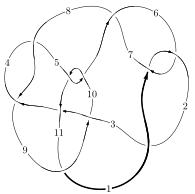
\includegraphics[width=112pt]{../../../GIT/diagram.site/Diagrams/png/467_11a_218.png}\\
\ \ \ A knot diagram\footnotemark}&
\allowdisplaybreaks
\textbf{Linearized knot diagam} \\
\cline{2-2}
 &
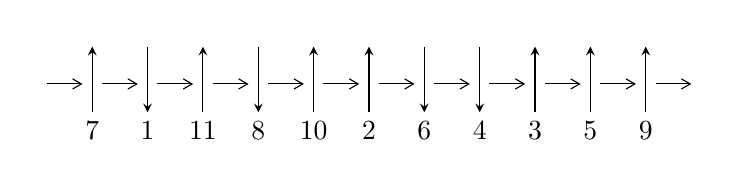
\begin{tikzpicture}[x=20pt, y=17pt]
	% nodes
	\node (C0) at (0, 0) {};
	\node (C1) at (1, 0) {};
	\node (C1U) at (1, +1) {};
	\node (C1D) at (1, -1) {7};

	\node (C2) at (2, 0) {};
	\node (C2U) at (2, +1) {};
	\node (C2D) at (2, -1) {1};

	\node (C3) at (3, 0) {};
	\node (C3U) at (3, +1) {};
	\node (C3D) at (3, -1) {11};

	\node (C4) at (4, 0) {};
	\node (C4U) at (4, +1) {};
	\node (C4D) at (4, -1) {8};

	\node (C5) at (5, 0) {};
	\node (C5U) at (5, +1) {};
	\node (C5D) at (5, -1) {10};

	\node (C6) at (6, 0) {};
	\node (C6U) at (6, +1) {};
	\node (C6D) at (6, -1) {2};

	\node (C7) at (7, 0) {};
	\node (C7U) at (7, +1) {};
	\node (C7D) at (7, -1) {6};

	\node (C8) at (8, 0) {};
	\node (C8U) at (8, +1) {};
	\node (C8D) at (8, -1) {4};

	\node (C9) at (9, 0) {};
	\node (C9U) at (9, +1) {};
	\node (C9D) at (9, -1) {3};

	\node (C10) at (10, 0) {};
	\node (C10U) at (10, +1) {};
	\node (C10D) at (10, -1) {5};

	\node (C11) at (11, 0) {};
	\node (C11U) at (11, +1) {};
	\node (C11D) at (11, -1) {9};
	\node (C12) at (12, 0) {};

	% arrows
	\draw[->,>={angle 60}]
	(C0) edge (C1) (C1) edge (C2) (C2) edge (C3) (C3) edge (C4) (C4) edge (C5) (C5) edge (C6) (C6) edge (C7) (C7) edge (C8) (C8) edge (C9) (C9) edge (C10) (C10) edge (C11) (C11) edge (C12) ;	\draw[->,>=stealth]
	(C1D) edge (C1U) (C2U) edge (C2D) (C3D) edge (C3U) (C4U) edge (C4D) (C5D) edge (C5U) (C6D) edge (C6U) (C7U) edge (C7D) (C8U) edge (C8D) (C9D) edge (C9U) (C10D) edge (C10U) (C11D) edge (C11U) ;
	\end{tikzpicture} \\
\hhline{~~} \\& 
\textbf{Solving Sequence} \\ \cline{2-2} 
 &
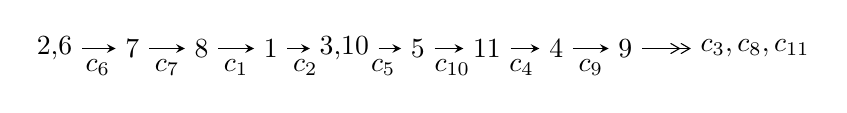
\begin{tikzpicture}[x=25pt, y=7pt]
	% node
	\node (A0) at (-1/8, 0) {2,6};
	\node (A1) at (1, 0) {7};
	\node (A2) at (2, 0) {8};
	\node (A3) at (3, 0) {1};
	\node (A4) at (65/16, 0) {3,10};
	\node (A5) at (41/8, 0) {5};
	\node (A6) at (49/8, 0) {11};
	\node (A7) at (57/8, 0) {4};
	\node (A8) at (65/8, 0) {9};
	\node (C1) at (1/2, -1) {$c_{6}$};
	\node (C2) at (3/2, -1) {$c_{7}$};
	\node (C3) at (5/2, -1) {$c_{1}$};
	\node (C4) at (7/2, -1) {$c_{2}$};
	\node (C5) at (37/8, -1) {$c_{5}$};
	\node (C6) at (45/8, -1) {$c_{10}$};
	\node (C7) at (53/8, -1) {$c_{4}$};
	\node (C8) at (61/8, -1) {$c_{9}$};
	\node (A9) at (10, 0) {$c_{3},c_{8},c_{11}$};

	% edge
	\draw[->,>=stealth]	
	(A0) edge (A1) (A1) edge (A2) (A2) edge (A3) (A3) edge (A4) (A4) edge (A5) (A5) edge (A6) (A6) edge (A7) (A7) edge (A8) ;
	\draw[->>,>={angle 60}]	
	(A8) edge (A9);
\end{tikzpicture} \\ 

\end{tabular} \\

\footnotetext{
The image of knot diagram is generated by the software ``\textbf{Draw programme}" developed by Andrew Bartholomew(\url{http://www.layer8.co.uk/maths/draw/index.htm\#Running-draw}), where we modified some parts for our purpose(\url{https://github.com/CATsTAILs/LinksPainter}).
}\phantom \\ \newline 
\centering \textbf{Ideals for irreducible components\footnotemark of $X_{\text{par}}$} 
 
\begin{align*}
I^u_{1}&=\langle 
-5.44804\times10^{62} u^{78}-1.03216\times10^{63} u^{77}+\cdots+3.63230\times10^{62} b+5.06666\times10^{63},\\
\phantom{I^u_{1}}&\phantom{= \langle  }-4.72952\times10^{63} u^{78}-1.07582\times10^{64} u^{77}+\cdots+2.54261\times10^{63} a+7.17584\times10^{64},\;u^{79}+u^{78}+\cdots-8 u-7\rangle \\
I^u_{2}&=\langle 
u^{11}+2 u^9+4 u^7- u^6+5 u^5- u^4+3 u^3- u^2+b+2 u,\\
\phantom{I^u_{2}}&\phantom{= \langle  }-2 u^{13}-2 u^{12}-6 u^{11}-5 u^{10}-14 u^9-9 u^8-19 u^7-11 u^6-19 u^5-8 u^4-13 u^3-7 u^2+a-5 u-2,\\
\phantom{I^u_{2}}&\phantom{= \langle  }u^{14}+3 u^{12}+7 u^{10}- u^9+11 u^8-2 u^7+12 u^6-3 u^5+10 u^4-2 u^3+5 u^2- u+1\rangle \\
\\
\end{align*}
\raggedright * 2 irreducible components of $\dim_{\mathbb{C}}=0$, with total 93 representations.\\
\footnotetext{All coefficients of polynomials are rational numbers. But the coefficients are sometimes approximated in decimal forms when there is not enough margin.}
\newpage
\renewcommand{\arraystretch}{1}
\centering \section*{I. $I^u_{1}= \langle -5.45\times10^{62} u^{78}-1.03\times10^{63} u^{77}+\cdots+3.63\times10^{62} b+5.07\times10^{63},\;-4.73\times10^{63} u^{78}-1.08\times10^{64} u^{77}+\cdots+2.54\times10^{63} a+7.18\times10^{64},\;u^{79}+u^{78}+\cdots-8 u-7 \rangle$}
\flushleft \textbf{(i) Arc colorings}\\
\begin{tabular}{m{7pt} m{180pt} m{7pt} m{180pt} }
\flushright $a_{2}=$&$\begin{pmatrix}0\\u\end{pmatrix}$ \\
\flushright $a_{6}=$&$\begin{pmatrix}1\\0\end{pmatrix}$ \\
\flushright $a_{7}=$&$\begin{pmatrix}1\\- u^2\end{pmatrix}$ \\
\flushright $a_{8}=$&$\begin{pmatrix}u^2+1\\- u^2\end{pmatrix}$ \\
\flushright $a_{1}=$&$\begin{pmatrix}- u\\u^3+u\end{pmatrix}$ \\
\flushright $a_{3}=$&$\begin{pmatrix}- u^3\\u^5+u^3+u\end{pmatrix}$ \\
\flushright $a_{10}=$&$\begin{pmatrix}1.86010 u^{78}+4.23115 u^{77}+\cdots-46.3492 u-28.2223\\1.49989 u^{78}+2.84161 u^{77}+\cdots-33.3985 u-13.9489\end{pmatrix}$ \\
\flushright $a_{5}=$&$\begin{pmatrix}1.17416 u^{78}+2.07095 u^{77}+\cdots-29.5282 u-10.3400\\0.206768 u^{78}-0.785482 u^{77}+\cdots+9.53356 u+11.2272\end{pmatrix}$ \\
\flushright $a_{11}=$&$\begin{pmatrix}-0.609104 u^{78}+0.369573 u^{77}+\cdots+8.80543 u-8.08874\\-1.73226 u^{78}-2.17804 u^{77}+\cdots+18.6211 u+2.73894\end{pmatrix}$ \\
\flushright $a_{4}=$&$\begin{pmatrix}1.64175 u^{78}+1.85665 u^{77}+\cdots-24.4203 u-9.52711\\-0.573692 u^{78}-2.27635 u^{77}+\cdots+22.8621 u+20.9732\end{pmatrix}$ \\
\flushright $a_{9}=$&$\begin{pmatrix}1.56053 u^{78}+3.29376 u^{77}+\cdots-36.4399 u-22.2196\\0.852462 u^{78}+1.64403 u^{77}+\cdots-21.4230 u-5.42602\end{pmatrix}$\\ \flushright $a_{9}=$&$\begin{pmatrix}1.56053 u^{78}+3.29376 u^{77}+\cdots-36.4399 u-22.2196\\0.852462 u^{78}+1.64403 u^{77}+\cdots-21.4230 u-5.42602\end{pmatrix}$\\&\end{tabular}
\flushleft \textbf{(ii) Obstruction class $= -1$}\\~\\
\flushleft \textbf{(iii) Cusp Shapes $= -2.57564 u^{78}-8.67107 u^{77}+\cdots+98.6500 u+77.0521$}\\~\\
\newpage\renewcommand{\arraystretch}{1}
\flushleft \textbf{(iv) u-Polynomials at the component}\newline \\
\begin{tabular}{m{50pt}|m{274pt}}
Crossings & \hspace{64pt}u-Polynomials at each crossing \\
\hline $$\begin{aligned}c_{1},c_{6}\end{aligned}$$&$\begin{aligned}
&u^{79}+u^{78}+\cdots-8 u-7
\end{aligned}$\\
\hline $$\begin{aligned}c_{2},c_{7}\end{aligned}$$&$\begin{aligned}
&u^{79}+25 u^{78}+\cdots-664 u-49
\end{aligned}$\\
\hline $$\begin{aligned}c_{3}\end{aligned}$$&$\begin{aligned}
&u^{79}+7 u^{78}+\cdots+2 u-1
\end{aligned}$\\
\hline $$\begin{aligned}c_{4},c_{8}\end{aligned}$$&$\begin{aligned}
&u^{79}-2 u^{78}+\cdots+347 u-71
\end{aligned}$\\
\hline $$\begin{aligned}c_{5},c_{10}\end{aligned}$$&$\begin{aligned}
&u^{79}- u^{78}+\cdots-14 u^2-1
\end{aligned}$\\
\hline $$\begin{aligned}c_{9}\end{aligned}$$&$\begin{aligned}
&u^{79}-5 u^{77}+\cdots-249 u-83
\end{aligned}$\\
\hline $$\begin{aligned}c_{11}\end{aligned}$$&$\begin{aligned}
&u^{79}+9 u^{78}+\cdots-4205 u-689
\end{aligned}$\\
\hline
\end{tabular}\\~\\
\newpage\renewcommand{\arraystretch}{1}
\flushleft \textbf{(v) Riley Polynomials at the component}\newline \\
\begin{tabular}{m{50pt}|m{274pt}}
Crossings & \hspace{64pt}Riley Polynomials at each crossing \\
\hline $$\begin{aligned}c_{1},c_{6}\end{aligned}$$&$\begin{aligned}
&y^{79}+25 y^{78}+\cdots-664 y-49
\end{aligned}$\\
\hline $$\begin{aligned}c_{2},c_{7}\end{aligned}$$&$\begin{aligned}
&y^{79}+65 y^{78}+\cdots+132784 y-2401
\end{aligned}$\\
\hline $$\begin{aligned}c_{3}\end{aligned}$$&$\begin{aligned}
&y^{79}-7 y^{78}+\cdots-10 y-1
\end{aligned}$\\
\hline $$\begin{aligned}c_{4},c_{8}\end{aligned}$$&$\begin{aligned}
&y^{79}+56 y^{78}+\cdots-115737 y-5041
\end{aligned}$\\
\hline $$\begin{aligned}c_{5},c_{10}\end{aligned}$$&$\begin{aligned}
&y^{79}+45 y^{78}+\cdots-28 y-1
\end{aligned}$\\
\hline $$\begin{aligned}c_{9}\end{aligned}$$&$\begin{aligned}
&y^{79}-10 y^{78}+\cdots+155127 y-6889
\end{aligned}$\\
\hline $$\begin{aligned}c_{11}\end{aligned}$$&$\begin{aligned}
&y^{79}-29 y^{78}+\cdots+14498845 y-474721
\end{aligned}$\\
\hline
\end{tabular}\\~\\
\newpage\flushleft \textbf{(vi) Complex Volumes and Cusp Shapes}
$$\begin{array}{c|c|c}  
\text{Solutions to }I^u_{1}& \I (\text{vol} + \sqrt{-1}CS) & \text{Cusp shape}\\
 \hline 
\begin{aligned}
u &= \phantom{-}0.068601 + 0.992204 I \\
a &= -0.153424 + 1.337650 I \\
b &= \phantom{-}0.691328 + 1.177290 I\end{aligned}
 & -3.14903 + 3.12627 I & \phantom{-0.000000 } 0 \\ \hline\begin{aligned}
u &= \phantom{-}0.068601 - 0.992204 I \\
a &= -0.153424 - 1.337650 I \\
b &= \phantom{-}0.691328 - 1.177290 I\end{aligned}
 & -3.14903 - 3.12627 I & \phantom{-0.000000 } 0 \\ \hline\begin{aligned}
u &= -0.747557 + 0.710223 I \\
a &= \phantom{-}1.241940 - 0.068757 I \\
b &= -0.468963 - 0.268238 I\end{aligned}
 & \phantom{-}3.61173 + 0.72947 I & \phantom{-0.000000 } 0 \\ \hline\begin{aligned}
u &= -0.747557 - 0.710223 I \\
a &= \phantom{-}1.241940 + 0.068757 I \\
b &= -0.468963 + 0.268238 I\end{aligned}
 & \phantom{-}3.61173 - 0.72947 I & \phantom{-0.000000 } 0 \\ \hline\begin{aligned}
u &= -0.718133 + 0.742230 I \\
a &= \phantom{-}1.30172 + 1.16845 I \\
b &= -0.996894 - 0.955293 I\end{aligned}
 & \phantom{-}2.13841 + 2.75328 I & \phantom{-0.000000 } 0 \\ \hline\begin{aligned}
u &= -0.718133 - 0.742230 I \\
a &= \phantom{-}1.30172 - 1.16845 I \\
b &= -0.996894 + 0.955293 I\end{aligned}
 & \phantom{-}2.13841 - 2.75328 I & \phantom{-0.000000 } 0 \\ \hline\begin{aligned}
u &= -0.385001 + 0.967084 I \\
a &= \phantom{-}0.856191 + 0.719727 I \\
b &= \phantom{-}0.062793 + 1.276180 I\end{aligned}
 & -4.88505 - 1.08505 I & \phantom{-0.000000 } 0 \\ \hline\begin{aligned}
u &= -0.385001 - 0.967084 I \\
a &= \phantom{-}0.856191 - 0.719727 I \\
b &= \phantom{-}0.062793 - 1.276180 I\end{aligned}
 & -4.88505 + 1.08505 I & \phantom{-0.000000 } 0 \\ \hline\begin{aligned}
u &= -0.236787 + 1.021880 I \\
a &= -1.30938 - 1.15749 I \\
b &= \phantom{-}0.300280 - 1.213660 I\end{aligned}
 & -5.62568 - 4.91714 I & \phantom{-0.000000 } 0 \\ \hline\begin{aligned}
u &= -0.236787 - 1.021880 I \\
a &= -1.30938 + 1.15749 I \\
b &= \phantom{-}0.300280 + 1.213660 I\end{aligned}
 & -5.62568 + 4.91714 I & \phantom{-0.000000 } 0\\
 \hline 
 \end{array}$$\newpage$$\begin{array}{c|c|c}  
\text{Solutions to }I^u_{1}& \I (\text{vol} + \sqrt{-1}CS) & \text{Cusp shape}\\
 \hline 
\begin{aligned}
u &= -0.294156 + 0.904371 I \\
a &= \phantom{-}0.0378805 - 0.1197230 I \\
b &= -0.979850 + 0.015955 I\end{aligned}
 & \phantom{-}1.42957 - 5.30340 I & \phantom{-0.000000 -}0. + 8.18949 I \\ \hline\begin{aligned}
u &= -0.294156 - 0.904371 I \\
a &= \phantom{-}0.0378805 + 0.1197230 I \\
b &= -0.979850 - 0.015955 I\end{aligned}
 & \phantom{-}1.42957 + 5.30340 I & \phantom{-0.000000 } 0. - 8.18949 I \\ \hline\begin{aligned}
u &= \phantom{-}0.725101 + 0.823158 I \\
a &= -0.364980 + 1.165740 I \\
b &= \phantom{-}0.586179 - 0.930088 I\end{aligned}
 & \phantom{-}0.91115 + 1.68888 I & \phantom{-0.000000 } 0 \\ \hline\begin{aligned}
u &= \phantom{-}0.725101 - 0.823158 I \\
a &= -0.364980 - 1.165740 I \\
b &= \phantom{-}0.586179 + 0.930088 I\end{aligned}
 & \phantom{-}0.91115 - 1.68888 I & \phantom{-0.000000 } 0 \\ \hline\begin{aligned}
u &= \phantom{-}0.588826 + 0.926444 I \\
a &= \phantom{-}0.999280 + 0.627418 I \\
b &= \phantom{-}0.259716 - 1.197850 I\end{aligned}
 & -0.22599 + 2.17222 I & \phantom{-0.000000 } 0 \\ \hline\begin{aligned}
u &= \phantom{-}0.588826 - 0.926444 I \\
a &= \phantom{-}0.999280 - 0.627418 I \\
b &= \phantom{-}0.259716 + 1.197850 I\end{aligned}
 & -0.22599 - 2.17222 I & \phantom{-0.000000 } 0 \\ \hline\begin{aligned}
u &= -0.710928 + 0.836978 I \\
a &= \phantom{-}2.18368 - 0.06877 I \\
b &= -0.286792 + 0.573885 I\end{aligned}
 & \phantom{-}3.19613 + 0.36905 I & \phantom{-0.000000 } 0 \\ \hline\begin{aligned}
u &= -0.710928 - 0.836978 I \\
a &= \phantom{-}2.18368 + 0.06877 I \\
b &= -0.286792 - 0.573885 I\end{aligned}
 & \phantom{-}3.19613 - 0.36905 I & \phantom{-0.000000 } 0 \\ \hline\begin{aligned}
u &= \phantom{-}0.106082 + 0.890241 I \\
a &= -0.369055 + 0.588099 I \\
b &= \phantom{-}0.565118 + 0.130913 I\end{aligned}
 & -1.64796 + 1.63173 I & -1.15356 - 4.67450 I \\ \hline\begin{aligned}
u &= \phantom{-}0.106082 - 0.890241 I \\
a &= -0.369055 - 0.588099 I \\
b &= \phantom{-}0.565118 - 0.130913 I\end{aligned}
 & -1.64796 - 1.63173 I & -1.15356 + 4.67450 I\\
 \hline 
 \end{array}$$\newpage$$\begin{array}{c|c|c}  
\text{Solutions to }I^u_{1}& \I (\text{vol} + \sqrt{-1}CS) & \text{Cusp shape}\\
 \hline 
\begin{aligned}
u &= \phantom{-}0.876569 + 0.066661 I \\
a &= -0.622530 - 0.556101 I \\
b &= \phantom{-}0.549607 + 1.031330 I\end{aligned}
 & \phantom{-}2.03962 + 6.66682 I & \phantom{-}6.74963 - 6.99085 I \\ \hline\begin{aligned}
u &= \phantom{-}0.876569 - 0.066661 I \\
a &= -0.622530 + 0.556101 I \\
b &= \phantom{-}0.549607 - 1.031330 I\end{aligned}
 & \phantom{-}2.03962 - 6.66682 I & \phantom{-}6.74963 + 6.99085 I \\ \hline\begin{aligned}
u &= \phantom{-}0.906807 + 0.666792 I \\
a &= -0.452346 + 0.331194 I \\
b &= \phantom{-}0.561743 - 1.084000 I\end{aligned}
 & \phantom{-}6.02916 - 1.41665 I & \phantom{-0.000000 } 0 \\ \hline\begin{aligned}
u &= \phantom{-}0.906807 - 0.666792 I \\
a &= -0.452346 - 0.331194 I \\
b &= \phantom{-}0.561743 + 1.084000 I\end{aligned}
 & \phantom{-}6.02916 + 1.41665 I & \phantom{-0.000000 } 0 \\ \hline\begin{aligned}
u &= -0.725122 + 0.874260 I \\
a &= -1.30561 + 0.72285 I \\
b &= -0.05188 - 1.88290 I\end{aligned}
 & -0.23925 - 2.76678 I & \phantom{-0.000000 } 0 \\ \hline\begin{aligned}
u &= -0.725122 - 0.874260 I \\
a &= -1.30561 - 0.72285 I \\
b &= -0.05188 + 1.88290 I\end{aligned}
 & -0.23925 + 2.76678 I & \phantom{-0.000000 } 0 \\ \hline\begin{aligned}
u &= \phantom{-}0.847566 + 0.759732 I \\
a &= \phantom{-}0.916382 - 0.975772 I \\
b &= -0.469786 + 1.039580 I\end{aligned}
 & \phantom{-}1.50890 - 3.98013 I & \phantom{-0.000000 } 0 \\ \hline\begin{aligned}
u &= \phantom{-}0.847566 - 0.759732 I \\
a &= \phantom{-}0.916382 + 0.975772 I \\
b &= -0.469786 - 1.039580 I\end{aligned}
 & \phantom{-}1.50890 + 3.98013 I & \phantom{-0.000000 } 0 \\ \hline\begin{aligned}
u &= \phantom{-}0.768818 + 0.842684 I \\
a &= \phantom{-}0.787145 - 0.216058 I \\
b &= -0.523775 + 1.132210 I\end{aligned}
 & \phantom{-}5.15403 - 0.95027 I & \phantom{-0.000000 } 0 \\ \hline\begin{aligned}
u &= \phantom{-}0.768818 - 0.842684 I \\
a &= \phantom{-}0.787145 + 0.216058 I \\
b &= -0.523775 - 1.132210 I\end{aligned}
 & \phantom{-}5.15403 + 0.95027 I & \phantom{-0.000000 } 0\\
 \hline 
 \end{array}$$\newpage$$\begin{array}{c|c|c}  
\text{Solutions to }I^u_{1}& \I (\text{vol} + \sqrt{-1}CS) & \text{Cusp shape}\\
 \hline 
\begin{aligned}
u &= \phantom{-}0.486696 + 0.703689 I \\
a &= \phantom{-}0.519465 + 0.821783 I \\
b &= \phantom{-}0.093122 - 0.577690 I\end{aligned}
 & \phantom{-}0.36304 + 1.84837 I & \phantom{-}2.66443 - 3.35239 I \\ \hline\begin{aligned}
u &= \phantom{-}0.486696 - 0.703689 I \\
a &= \phantom{-}0.519465 - 0.821783 I \\
b &= \phantom{-}0.093122 + 0.577690 I\end{aligned}
 & \phantom{-}0.36304 - 1.84837 I & \phantom{-}2.66443 + 3.35239 I \\ \hline\begin{aligned}
u &= \phantom{-}0.843432 + 0.790066 I \\
a &= -1.72508 + 0.39273 I \\
b &= \phantom{-}1.287590 + 0.433064 I\end{aligned}
 & \phantom{-}8.57301 - 3.45586 I & \phantom{-0.000000 } 0 \\ \hline\begin{aligned}
u &= \phantom{-}0.843432 - 0.790066 I \\
a &= -1.72508 - 0.39273 I \\
b &= \phantom{-}1.287590 - 0.433064 I\end{aligned}
 & \phantom{-}8.57301 + 3.45586 I & \phantom{-0.000000 } 0 \\ \hline\begin{aligned}
u &= -0.909408 + 0.715797 I \\
a &= -0.822486 - 0.850087 I \\
b &= \phantom{-}0.75301 + 1.25876 I\end{aligned}
 & \phantom{-}5.89486 + 10.51700 I & \phantom{-0.000000 } 0 \\ \hline\begin{aligned}
u &= -0.909408 - 0.715797 I \\
a &= -0.822486 + 0.850087 I \\
b &= \phantom{-}0.75301 - 1.25876 I\end{aligned}
 & \phantom{-}5.89486 - 10.51700 I & \phantom{-0.000000 } 0 \\ \hline\begin{aligned}
u &= -0.709662 + 0.915793 I \\
a &= -1.23890 - 0.75698 I \\
b &= \phantom{-}0.452617 + 0.379590 I\end{aligned}
 & \phantom{-}2.94594 - 5.81075 I & \phantom{-0.000000 } 0 \\ \hline\begin{aligned}
u &= -0.709662 - 0.915793 I \\
a &= -1.23890 + 0.75698 I \\
b &= \phantom{-}0.452617 - 0.379590 I\end{aligned}
 & \phantom{-}2.94594 + 5.81075 I & \phantom{-0.000000 } 0 \\ \hline\begin{aligned}
u &= \phantom{-}0.724913 + 0.913338 I \\
a &= \phantom{-}1.94129 + 0.25721 I \\
b &= -0.615371 - 1.136900 I\end{aligned}
 & \phantom{-}0.63787 + 3.85193 I & \phantom{-0.000000 } 0 \\ \hline\begin{aligned}
u &= \phantom{-}0.724913 - 0.913338 I \\
a &= \phantom{-}1.94129 - 0.25721 I \\
b &= -0.615371 + 1.136900 I\end{aligned}
 & \phantom{-}0.63787 - 3.85193 I & \phantom{-0.000000 } 0\\
 \hline 
 \end{array}$$\newpage$$\begin{array}{c|c|c}  
\text{Solutions to }I^u_{1}& \I (\text{vol} + \sqrt{-1}CS) & \text{Cusp shape}\\
 \hline 
\begin{aligned}
u &= \phantom{-}0.272193 + 1.148200 I \\
a &= \phantom{-}0.673138 - 1.136890 I \\
b &= -0.539494 - 1.221250 I\end{aligned}
 & -2.11575 + 10.45870 I & \phantom{-0.000000 } 0 \\ \hline\begin{aligned}
u &= \phantom{-}0.272193 - 1.148200 I \\
a &= \phantom{-}0.673138 + 1.136890 I \\
b &= -0.539494 + 1.221250 I\end{aligned}
 & -2.11575 - 10.45870 I & \phantom{-0.000000 } 0 \\ \hline\begin{aligned}
u &= \phantom{-}0.752269 + 0.913216 I \\
a &= -2.08253 + 0.73148 I \\
b &= \phantom{-}0.449175 + 1.172200 I\end{aligned}
 & \phantom{-}4.93567 + 6.70197 I & \phantom{-0.000000 } 0 \\ \hline\begin{aligned}
u &= \phantom{-}0.752269 - 0.913216 I \\
a &= -2.08253 - 0.73148 I \\
b &= \phantom{-}0.449175 - 1.172200 I\end{aligned}
 & \phantom{-}4.93567 - 6.70197 I & \phantom{-0.000000 } 0 \\ \hline\begin{aligned}
u &= -0.699416 + 0.965229 I \\
a &= -2.35631 - 0.61292 I \\
b &= \phantom{-}1.00524 - 1.09298 I\end{aligned}
 & \phantom{-}1.46348 - 8.20122 I & \phantom{-0.000000 } 0 \\ \hline\begin{aligned}
u &= -0.699416 - 0.965229 I \\
a &= -2.35631 + 0.61292 I \\
b &= \phantom{-}1.00524 + 1.09298 I\end{aligned}
 & \phantom{-}1.46348 + 8.20122 I & \phantom{-0.000000 } 0 \\ \hline\begin{aligned}
u &= -0.088492 + 0.800040 I \\
a &= \phantom{-}0.66008 - 3.50543 I \\
b &= \phantom{-}0.198364 - 0.926764 I\end{aligned}
 & \phantom{-}0.06134 - 3.40830 I & \phantom{-}0.00748 + 5.95558 I \\ \hline\begin{aligned}
u &= -0.088492 - 0.800040 I \\
a &= \phantom{-}0.66008 + 3.50543 I \\
b &= \phantom{-}0.198364 + 0.926764 I\end{aligned}
 & \phantom{-}0.06134 + 3.40830 I & \phantom{-}0.00748 - 5.95558 I \\ \hline\begin{aligned}
u &= -0.072534 + 1.193830 I \\
a &= -0.178921 + 1.190570 I \\
b &= -0.263590 + 0.843873 I\end{aligned}
 & -1.193530 - 0.319368 I & \phantom{-0.000000 } 0 \\ \hline\begin{aligned}
u &= -0.072534 - 1.193830 I \\
a &= -0.178921 - 1.190570 I \\
b &= -0.263590 - 0.843873 I\end{aligned}
 & -1.193530 + 0.319368 I & \phantom{-0.000000 } 0\\
 \hline 
 \end{array}$$\newpage$$\begin{array}{c|c|c}  
\text{Solutions to }I^u_{1}& \I (\text{vol} + \sqrt{-1}CS) & \text{Cusp shape}\\
 \hline 
\begin{aligned}
u &= -0.056663 + 0.795280 I \\
a &= \phantom{-}1.07684 + 1.56691 I \\
b &= -0.23874 + 1.54232 I\end{aligned}
 & -3.94909 - 0.33166 I & -2.88323 - 2.20171 I \\ \hline\begin{aligned}
u &= -0.056663 - 0.795280 I \\
a &= \phantom{-}1.07684 - 1.56691 I \\
b &= -0.23874 - 1.54232 I\end{aligned}
 & -3.94909 + 0.33166 I & -2.88323 + 2.20171 I \\ \hline\begin{aligned}
u &= -0.688272 + 0.999750 I \\
a &= -1.40266 - 0.69035 I \\
b &= \phantom{-}0.347900 - 0.472595 I\end{aligned}
 & \phantom{-}2.72299 - 6.21170 I & \phantom{-0.000000 } 0 \\ \hline\begin{aligned}
u &= -0.688272 - 0.999750 I \\
a &= -1.40266 + 0.69035 I \\
b &= \phantom{-}0.347900 + 0.472595 I\end{aligned}
 & \phantom{-}2.72299 + 6.21170 I & \phantom{-0.000000 } 0 \\ \hline\begin{aligned}
u &= \phantom{-}0.778280 + 0.975214 I \\
a &= \phantom{-}1.04179 - 1.15319 I \\
b &= -1.356540 + 0.352012 I\end{aligned}
 & \phantom{-}7.99698 + 9.50667 I & \phantom{-0.000000 } 0 \\ \hline\begin{aligned}
u &= \phantom{-}0.778280 - 0.975214 I \\
a &= \phantom{-}1.04179 + 1.15319 I \\
b &= -1.356540 - 0.352012 I\end{aligned}
 & \phantom{-}7.99698 - 9.50667 I & \phantom{-0.000000 } 0 \\ \hline\begin{aligned}
u &= -0.903504 + 0.861547 I \\
a &= -0.660376 - 0.226832 I \\
b &= \phantom{-}0.502624 - 0.303555 I\end{aligned}
 & \phantom{-}8.16830 - 3.10045 I & \phantom{-0.000000 } 0 \\ \hline\begin{aligned}
u &= -0.903504 - 0.861547 I \\
a &= -0.660376 + 0.226832 I \\
b &= \phantom{-}0.502624 + 0.303555 I\end{aligned}
 & \phantom{-}8.16830 + 3.10045 I & \phantom{-0.000000 } 0 \\ \hline\begin{aligned}
u &= \phantom{-}0.347261 + 1.209130 I \\
a &= -0.622118 + 0.380504 I \\
b &= -0.341064 + 0.969919 I\end{aligned}
 & -1.76986 - 2.28307 I & \phantom{-0.000000 } 0 \\ \hline\begin{aligned}
u &= \phantom{-}0.347261 - 1.209130 I \\
a &= -0.622118 - 0.380504 I \\
b &= -0.341064 - 0.969919 I\end{aligned}
 & -1.76986 + 2.28307 I & \phantom{-0.000000 } 0\\
 \hline 
 \end{array}$$\newpage$$\begin{array}{c|c|c}  
\text{Solutions to }I^u_{1}& \I (\text{vol} + \sqrt{-1}CS) & \text{Cusp shape}\\
 \hline 
\begin{aligned}
u &= \phantom{-}0.768557 + 0.996208 I \\
a &= -2.12255 - 0.03776 I \\
b &= \phantom{-}0.508968 + 1.098010 I\end{aligned}
 & \phantom{-}0.77749 + 10.01260 I & \phantom{-0.000000 } 0 \\ \hline\begin{aligned}
u &= \phantom{-}0.768557 - 0.996208 I \\
a &= -2.12255 + 0.03776 I \\
b &= \phantom{-}0.508968 - 1.098010 I\end{aligned}
 & \phantom{-}0.77749 - 10.01260 I & \phantom{-0.000000 } 0 \\ \hline\begin{aligned}
u &= -0.865083 + 0.914831 I \\
a &= \phantom{-}0.162002 - 0.696670 I \\
b &= \phantom{-}0.026697 + 0.290718 I\end{aligned}
 & \phantom{-}7.97266 - 3.20478 I & \phantom{-0.000000 } 0 \\ \hline\begin{aligned}
u &= -0.865083 - 0.914831 I \\
a &= \phantom{-}0.162002 + 0.696670 I \\
b &= \phantom{-}0.026697 - 0.290718 I\end{aligned}
 & \phantom{-}7.97266 + 3.20478 I & \phantom{-0.000000 } 0 \\ \hline\begin{aligned}
u &= -0.842928 + 0.946030 I \\
a &= \phantom{-}0.590128 + 0.065077 I \\
b &= -0.541177 - 0.008044 I\end{aligned}
 & \phantom{-}7.88914 - 3.32695 I & \phantom{-0.000000 } 0 \\ \hline\begin{aligned}
u &= -0.842928 - 0.946030 I \\
a &= \phantom{-}0.590128 - 0.065077 I \\
b &= -0.541177 + 0.008044 I\end{aligned}
 & \phantom{-}7.88914 + 3.32695 I & \phantom{-0.000000 } 0 \\ \hline\begin{aligned}
u &= -0.668593 + 0.213008 I \\
a &= -0.641632 - 0.638273 I \\
b &= \phantom{-}0.657782 - 0.479809 I\end{aligned}
 & \phantom{-}3.63016 + 1.97736 I & \phantom{-}9.76414 - 0.88731 I \\ \hline\begin{aligned}
u &= -0.668593 - 0.213008 I \\
a &= -0.641632 + 0.638273 I \\
b &= \phantom{-}0.657782 + 0.479809 I\end{aligned}
 & \phantom{-}3.63016 - 1.97736 I & \phantom{-}9.76414 + 0.88731 I \\ \hline\begin{aligned}
u &= -0.776485 + 1.042220 I \\
a &= \phantom{-}2.05300 + 0.37394 I \\
b &= -0.74638 + 1.32056 I\end{aligned}
 & \phantom{-}4.8754 - 16.7440 I & \phantom{-0.000000 } 0 \\ \hline\begin{aligned}
u &= -0.776485 - 1.042220 I \\
a &= \phantom{-}2.05300 - 0.37394 I \\
b &= -0.74638 - 1.32056 I\end{aligned}
 & \phantom{-}4.8754 + 16.7440 I & \phantom{-0.000000 } 0\\
 \hline 
 \end{array}$$\newpage$$\begin{array}{c|c|c}  
\text{Solutions to }I^u_{1}& \I (\text{vol} + \sqrt{-1}CS) & \text{Cusp shape}\\
 \hline 
\begin{aligned}
u &= \phantom{-}0.762838 + 1.065990 I \\
a &= \phantom{-}1.46928 - 0.52381 I \\
b &= -0.495147 - 1.185170 I\end{aligned}
 & \phantom{-}4.80363 + 7.58954 I & \phantom{-0.000000 } 0 \\ \hline\begin{aligned}
u &= \phantom{-}0.762838 - 1.065990 I \\
a &= \phantom{-}1.46928 + 0.52381 I \\
b &= -0.495147 + 1.185170 I\end{aligned}
 & \phantom{-}4.80363 - 7.58954 I & \phantom{-0.000000 } 0 \\ \hline\begin{aligned}
u &= \phantom{-}0.482336 + 0.441392 I \\
a &= \phantom{-}1.20543 + 0.91074 I \\
b &= -0.492152 - 0.878703 I\end{aligned}
 & \phantom{-}0.81950 + 2.03003 I & \phantom{-}6.05353 - 3.33812 I \\ \hline\begin{aligned}
u &= \phantom{-}0.482336 - 0.441392 I \\
a &= \phantom{-}1.20543 - 0.91074 I \\
b &= -0.492152 + 0.878703 I\end{aligned}
 & \phantom{-}0.81950 - 2.03003 I & \phantom{-}6.05353 + 3.33812 I \\ \hline\begin{aligned}
u &= -0.596765 + 0.028691 I \\
a &= \phantom{-}0.787991 - 1.060340 I \\
b &= -0.142905 + 1.090580 I\end{aligned}
 & -2.35254 - 2.09310 I & \phantom{-}1.61759 + 3.77424 I \\ \hline\begin{aligned}
u &= -0.596765 - 0.028691 I \\
a &= \phantom{-}0.787991 + 1.060340 I \\
b &= -0.142905 - 1.090580 I\end{aligned}
 & -2.35254 + 2.09310 I & \phantom{-}1.61759 - 3.77424 I \\ \hline\begin{aligned}
u &= -0.119202 + 0.475498 I \\
a &= \phantom{-}2.06498 + 0.81754 I \\
b &= -0.577638 - 0.808331 I\end{aligned}
 & \phantom{-}0.98268 + 2.41658 I & \phantom{-}3.66259 + 0.85361 I \\ \hline\begin{aligned}
u &= -0.119202 - 0.475498 I \\
a &= \phantom{-}2.06498 - 0.81754 I \\
b &= -0.577638 + 0.808331 I\end{aligned}
 & \phantom{-}0.98268 - 2.41658 I & \phantom{-}3.66259 - 0.85361 I \\ \hline\begin{aligned}
u &= \phantom{-}0.415093\phantom{ +0.000000I} \\
a &= \phantom{-}1.43678\phantom{ +0.000000I} \\
b &= -0.463470\phantom{ +0.000000I}\end{aligned}
 & \phantom{-}0.930718\phantom{ +0.000000I} & \phantom{-}11.0930\phantom{ +0.000000I}\\
 \hline 
 \end{array}$$\newpage\newpage\renewcommand{\arraystretch}{1}
\centering \section*{II. $I^u_{2}= \langle u^{11}+2 u^9+\cdots+b+2 u,\;-2 u^{13}-2 u^{12}+\cdots+a-2,\;u^{14}+3 u^{12}+\cdots- u+1 \rangle$}
\flushleft \textbf{(i) Arc colorings}\\
\begin{tabular}{m{7pt} m{180pt} m{7pt} m{180pt} }
\flushright $a_{2}=$&$\begin{pmatrix}0\\u\end{pmatrix}$ \\
\flushright $a_{6}=$&$\begin{pmatrix}1\\0\end{pmatrix}$ \\
\flushright $a_{7}=$&$\begin{pmatrix}1\\- u^2\end{pmatrix}$ \\
\flushright $a_{8}=$&$\begin{pmatrix}u^2+1\\- u^2\end{pmatrix}$ \\
\flushright $a_{1}=$&$\begin{pmatrix}- u\\u^3+u\end{pmatrix}$ \\
\flushright $a_{3}=$&$\begin{pmatrix}- u^3\\u^5+u^3+u\end{pmatrix}$ \\
\flushright $a_{10}=$&$\begin{pmatrix}2 u^{13}+2 u^{12}+\cdots+5 u+2\\- u^{11}-2 u^9-4 u^7+u^6-5 u^5+u^4-3 u^3+u^2-2 u\end{pmatrix}$ \\
\flushright $a_{5}=$&$\begin{pmatrix}-3 u^{13}+u^{12}+\cdots-6 u+3\\u^{12}+3 u^{10}+7 u^8- u^7+10 u^6-2 u^5+10 u^4-3 u^3+7 u^2- u+1\end{pmatrix}$ \\
\flushright $a_{11}=$&$\begin{pmatrix}2 u^{13}+u^{12}+\cdots+4 u-1\\- u^{13}- u^{12}+\cdots- u-1\end{pmatrix}$ \\
\flushright $a_{4}=$&$\begin{pmatrix}-2 u^{13}+u^{12}+\cdots-3 u+2\\u^{12}+3 u^{10}+7 u^8- u^7+10 u^6- u^5+10 u^4-2 u^3+7 u^2+1\end{pmatrix}$ \\
\flushright $a_{9}=$&$\begin{pmatrix}2 u^{13}+u^{12}+\cdots+6 u+1\\- u^{11}-2 u^9- u^8-4 u^7- u^6-5 u^5-2 u^4-3 u^3-2 u^2-2 u-1\end{pmatrix}$\\ \flushright $a_{9}=$&$\begin{pmatrix}2 u^{13}+u^{12}+\cdots+6 u+1\\- u^{11}-2 u^9- u^8-4 u^7- u^6-5 u^5-2 u^4-3 u^3-2 u^2-2 u-1\end{pmatrix}$\\&\end{tabular}
\flushleft \textbf{(ii) Obstruction class $= 1$}\\~\\
\flushleft \textbf{(iii) Cusp Shapes $= -8 u^{13}-3 u^{12}-22 u^{11}-9 u^{10}-53 u^9-13 u^8-77 u^7-16 u^6-79 u^5-6 u^4-61 u^3-9 u^2-21 u+3$}\\~\\
\newpage\renewcommand{\arraystretch}{1}
\flushleft \textbf{(iv) u-Polynomials at the component}\newline \\
\begin{tabular}{m{50pt}|m{274pt}}
Crossings & \hspace{64pt}u-Polynomials at each crossing \\
\hline $$\begin{aligned}c_{1}\end{aligned}$$&$\begin{aligned}
&u^{14}+3 u^{12}+\cdots+u+1
\end{aligned}$\\
\hline $$\begin{aligned}c_{2},c_{7}\end{aligned}$$&$\begin{aligned}
&u^{14}+6 u^{13}+\cdots+9 u+1
\end{aligned}$\\
\hline $$\begin{aligned}c_{3}\end{aligned}$$&$\begin{aligned}
&u^{14}+2 u^{13}+u^{12}-2 u^{10}-4 u^9+2 u^8+u^6+3 u^5-3 u^4- u+1
\end{aligned}$\\
\hline $$\begin{aligned}c_{4}\end{aligned}$$&$\begin{aligned}
&u^{14}- u^{13}+\cdots+7 u^2+1
\end{aligned}$\\
\hline $$\begin{aligned}c_{5}\end{aligned}$$&$\begin{aligned}
&u^{14}+7 u^{12}+\cdots+u+1
\end{aligned}$\\
\hline $$\begin{aligned}c_{6}\end{aligned}$$&$\begin{aligned}
&u^{14}+3 u^{12}+\cdots- u+1
\end{aligned}$\\
\hline $$\begin{aligned}c_{8}\end{aligned}$$&$\begin{aligned}
&u^{14}+u^{13}+\cdots+7 u^2+1
\end{aligned}$\\
\hline $$\begin{aligned}c_{9}\end{aligned}$$&$\begin{aligned}
&u^{14}+u^{13}-3 u^{10}-3 u^9+u^8+2 u^6+4 u^5-2 u^4+u^2-2 u+1
\end{aligned}$\\
\hline $$\begin{aligned}c_{10}\end{aligned}$$&$\begin{aligned}
&u^{14}+7 u^{12}+\cdots- u+1
\end{aligned}$\\
\hline $$\begin{aligned}c_{11}\end{aligned}$$&$\begin{aligned}
&u^{14}-4 u^{12}+\cdots-6 u+1
\end{aligned}$\\
\hline
\end{tabular}\\~\\
\newpage\renewcommand{\arraystretch}{1}
\flushleft \textbf{(v) Riley Polynomials at the component}\newline \\
\begin{tabular}{m{50pt}|m{274pt}}
Crossings & \hspace{64pt}Riley Polynomials at each crossing \\
\hline $$\begin{aligned}c_{1},c_{6}\end{aligned}$$&$\begin{aligned}
&y^{14}+6 y^{13}+\cdots+9 y+1
\end{aligned}$\\
\hline $$\begin{aligned}c_{2},c_{7}\end{aligned}$$&$\begin{aligned}
&y^{14}+10 y^{13}+\cdots+y+1
\end{aligned}$\\
\hline $$\begin{aligned}c_{3}\end{aligned}$$&$\begin{aligned}
&y^{14}-2 y^{13}+\cdots- y+1
\end{aligned}$\\
\hline $$\begin{aligned}c_{4},c_{8}\end{aligned}$$&$\begin{aligned}
&y^{14}+13 y^{13}+\cdots+14 y+1
\end{aligned}$\\
\hline $$\begin{aligned}c_{5},c_{10}\end{aligned}$$&$\begin{aligned}
&y^{14}+14 y^{13}+\cdots+13 y+1
\end{aligned}$\\
\hline $$\begin{aligned}c_{9}\end{aligned}$$&$\begin{aligned}
&y^{14}- y^{13}+\cdots-2 y+1
\end{aligned}$\\
\hline $$\begin{aligned}c_{11}\end{aligned}$$&$\begin{aligned}
&y^{14}-8 y^{13}+\cdots-4 y+1
\end{aligned}$\\
\hline
\end{tabular}\\~\\
\newpage\flushleft \textbf{(vi) Complex Volumes and Cusp Shapes}
$$\begin{array}{c|c|c}  
\text{Solutions to }I^u_{2}& \I (\text{vol} + \sqrt{-1}CS) & \text{Cusp shape}\\
 \hline 
\begin{aligned}
u &= \phantom{-}0.726429 + 0.738003 I \\
a &= \phantom{-}1.353070 - 0.241803 I \\
b &= -0.584789 + 0.795162 I\end{aligned}
 & \phantom{-}3.27925 - 1.94202 I & \phantom{-}6.99263 + 3.48916 I \\ \hline\begin{aligned}
u &= \phantom{-}0.726429 - 0.738003 I \\
a &= \phantom{-}1.353070 + 0.241803 I \\
b &= -0.584789 - 0.795162 I\end{aligned}
 & \phantom{-}3.27925 + 1.94202 I & \phantom{-}6.99263 - 3.48916 I \\ \hline\begin{aligned}
u &= -0.653577 + 0.866508 I \\
a &= \phantom{-}1.42775 - 1.02270 I \\
b &= \phantom{-}0.04408 + 1.69162 I\end{aligned}
 & -1.39544 - 2.54104 I & -3.53419 + 2.88773 I \\ \hline\begin{aligned}
u &= -0.653577 - 0.866508 I \\
a &= \phantom{-}1.42775 + 1.02270 I \\
b &= \phantom{-}0.04408 - 1.69162 I\end{aligned}
 & -1.39544 + 2.54104 I & -3.53419 - 2.88773 I \\ \hline\begin{aligned}
u &= -0.252602 + 0.846708 I \\
a &= -0.614186 - 1.257430 I \\
b &= \phantom{-}0.10455 - 1.45717 I\end{aligned}
 & -3.69976 - 1.12261 I & \phantom{-}2.04246 + 5.85401 I \\ \hline\begin{aligned}
u &= -0.252602 - 0.846708 I \\
a &= -0.614186 + 1.257430 I \\
b &= \phantom{-}0.10455 + 1.45717 I\end{aligned}
 & -3.69976 + 1.12261 I & \phantom{-}2.04246 - 5.85401 I \\ \hline\begin{aligned}
u &= \phantom{-}0.164460 + 1.120840 I \\
a &= \phantom{-}0.734317 - 1.077060 I \\
b &= \phantom{-}0.258541 - 0.856843 I\end{aligned}
 & -1.23971 - 1.45474 I & \phantom{-}3.50312 + 2.29074 I \\ \hline\begin{aligned}
u &= \phantom{-}0.164460 - 1.120840 I \\
a &= \phantom{-}0.734317 + 1.077060 I \\
b &= \phantom{-}0.258541 + 0.856843 I\end{aligned}
 & -1.23971 + 1.45474 I & \phantom{-}3.50312 - 2.29074 I \\ \hline\begin{aligned}
u &= \phantom{-}0.693530 + 0.982336 I \\
a &= -1.97340 + 0.86184 I \\
b &= \phantom{-}0.590972 + 0.911227 I\end{aligned}
 & \phantom{-}2.52164 + 7.39185 I & \phantom{-}5.20313 - 8.53818 I \\ \hline\begin{aligned}
u &= \phantom{-}0.693530 - 0.982336 I \\
a &= -1.97340 - 0.86184 I \\
b &= \phantom{-}0.590972 - 0.911227 I\end{aligned}
 & \phantom{-}2.52164 - 7.39185 I & \phantom{-}5.20313 + 8.53818 I\\
 \hline 
 \end{array}$$\newpage$$\begin{array}{c|c|c}  
\text{Solutions to }I^u_{2}& \I (\text{vol} + \sqrt{-1}CS) & \text{Cusp shape}\\
 \hline 
\begin{aligned}
u &= -0.890932 + 0.918447 I \\
a &= \phantom{-}0.306117 - 0.672539 I \\
b &= -0.035727 + 0.562759 I\end{aligned}
 & \phantom{-}7.64720 - 3.27992 I & -7.30018 + 4.84584 I \\ \hline\begin{aligned}
u &= -0.890932 - 0.918447 I \\
a &= \phantom{-}0.306117 + 0.672539 I \\
b &= -0.035727 - 0.562759 I\end{aligned}
 & \phantom{-}7.64720 + 3.27992 I & -7.30018 - 4.84584 I \\ \hline\begin{aligned}
u &= \phantom{-}0.212692 + 0.537116 I \\
a &= \phantom{-}0.26634 + 2.51077 I \\
b &= -0.377626 - 0.645284 I\end{aligned}
 & \phantom{-}1.11150 + 3.22050 I & \phantom{-}7.09303 - 7.62197 I \\ \hline\begin{aligned}
u &= \phantom{-}0.212692 - 0.537116 I \\
a &= \phantom{-}0.26634 - 2.51077 I \\
b &= -0.377626 + 0.645284 I\end{aligned}
 & \phantom{-}1.11150 - 3.22050 I & \phantom{-}7.09303 + 7.62197 I\\
 \hline 
 \end{array}$$\newpage
\newpage\renewcommand{\arraystretch}{1}
\centering \section*{ III. u-Polynomials}
\begin{tabular}{m{50pt}|m{274pt}}
Crossings & \hspace{64pt}u-Polynomials at each crossing \\
\hline $$\begin{aligned}c_{1}\end{aligned}$$&$\begin{aligned}
&(u^{14}+3 u^{12}+\cdots+u+1)(u^{79}+u^{78}+\cdots-8 u-7)
\end{aligned}$\\
\hline $$\begin{aligned}c_{2},c_{7}\end{aligned}$$&$\begin{aligned}
&(u^{14}+6 u^{13}+\cdots+9 u+1)(u^{79}+25 u^{78}+\cdots-664 u-49)
\end{aligned}$\\
\hline $$\begin{aligned}c_{3}\end{aligned}$$&$\begin{aligned}
&(u^{14}+2 u^{13}+u^{12}-2 u^{10}-4 u^9+2 u^8+u^6+3 u^5-3 u^4- u+1)\\
&\cdot(u^{79}+7 u^{78}+\cdots+2 u-1)
\end{aligned}$\\
\hline $$\begin{aligned}c_{4}\end{aligned}$$&$\begin{aligned}
&(u^{14}- u^{13}+\cdots+7 u^2+1)(u^{79}-2 u^{78}+\cdots+347 u-71)
\end{aligned}$\\
\hline $$\begin{aligned}c_{5}\end{aligned}$$&$\begin{aligned}
&(u^{14}+7 u^{12}+\cdots+u+1)(u^{79}- u^{78}+\cdots-14 u^2-1)
\end{aligned}$\\
\hline $$\begin{aligned}c_{6}\end{aligned}$$&$\begin{aligned}
&(u^{14}+3 u^{12}+\cdots- u+1)(u^{79}+u^{78}+\cdots-8 u-7)
\end{aligned}$\\
\hline $$\begin{aligned}c_{8}\end{aligned}$$&$\begin{aligned}
&(u^{14}+u^{13}+\cdots+7 u^2+1)(u^{79}-2 u^{78}+\cdots+347 u-71)
\end{aligned}$\\
\hline $$\begin{aligned}c_{9}\end{aligned}$$&$\begin{aligned}
&(u^{14}+u^{13}-3 u^{10}-3 u^9+u^8+2 u^6+4 u^5-2 u^4+u^2-2 u+1)\\
&\cdot(u^{79}-5 u^{77}+\cdots-249 u-83)
\end{aligned}$\\
\hline $$\begin{aligned}c_{10}\end{aligned}$$&$\begin{aligned}
&(u^{14}+7 u^{12}+\cdots- u+1)(u^{79}- u^{78}+\cdots-14 u^2-1)
\end{aligned}$\\
\hline $$\begin{aligned}c_{11}\end{aligned}$$&$\begin{aligned}
&(u^{14}-4 u^{12}+\cdots-6 u+1)(u^{79}+9 u^{78}+\cdots-4205 u-689)
\end{aligned}$\\
\hline
\end{tabular}\newpage\renewcommand{\arraystretch}{1}
\centering \section*{ IV. Riley Polynomials}
\begin{tabular}{m{50pt}|m{274pt}}
Crossings & \hspace{64pt}Riley Polynomials at each crossing \\
\hline $$\begin{aligned}c_{1},c_{6}\end{aligned}$$&$\begin{aligned}
&(y^{14}+6 y^{13}+\cdots+9 y+1)(y^{79}+25 y^{78}+\cdots-664 y-49)
\end{aligned}$\\
\hline $$\begin{aligned}c_{2},c_{7}\end{aligned}$$&$\begin{aligned}
&(y^{14}+10 y^{13}+\cdots+y+1)(y^{79}+65 y^{78}+\cdots+132784 y-2401)
\end{aligned}$\\
\hline $$\begin{aligned}c_{3}\end{aligned}$$&$\begin{aligned}
&(y^{14}-2 y^{13}+\cdots- y+1)(y^{79}-7 y^{78}+\cdots-10 y-1)
\end{aligned}$\\
\hline $$\begin{aligned}c_{4},c_{8}\end{aligned}$$&$\begin{aligned}
&(y^{14}+13 y^{13}+\cdots+14 y+1)(y^{79}+56 y^{78}+\cdots-115737 y-5041)
\end{aligned}$\\
\hline $$\begin{aligned}c_{5},c_{10}\end{aligned}$$&$\begin{aligned}
&(y^{14}+14 y^{13}+\cdots+13 y+1)(y^{79}+45 y^{78}+\cdots-28 y-1)
\end{aligned}$\\
\hline $$\begin{aligned}c_{9}\end{aligned}$$&$\begin{aligned}
&(y^{14}- y^{13}+\cdots-2 y+1)(y^{79}-10 y^{78}+\cdots+155127 y-6889)
\end{aligned}$\\
\hline $$\begin{aligned}c_{11}\end{aligned}$$&$\begin{aligned}
&(y^{14}-8 y^{13}+\cdots-4 y+1)(y^{79}-29 y^{78}+\cdots+1.44988\times10^{7} y-474721)
\end{aligned}$\\
\hline
\end{tabular}
\vskip 2pc
\end{document}